\documentclass[xcolor=pdftex,dvipsnames,table,mathserif,aspectratio=169]{beamer}
\usetheme{metropolis}
%\usetheme{Darmstadt}
%\usepackage{times}
%\usefonttheme{structurebold}

\usepackage[english]{babel}
%\usepackage[table]{xcolor}
\usepackage{pgf,pgfarrows,pgfnodes,pgfautomata,pgfheaps}
\usepackage{amsmath,amssymb,setspace}
\usepackage[latin1]{inputenc}
\usepackage[T1]{fontenc}
\usepackage{relsize}
\usepackage[absolute,overlay]{textpos}
\newenvironment{reference}[2]{%
  \begin{textblock*}{\textwidth}(#1,#2)
      \footnotesize\it\bgroup\color{red!50!black}}{\egroup\end{textblock*}}

\DeclareMathSizes{10}{10}{6}{6}


\title{Representative Consumer Models}
\author{C.Conlon}
\institute{Grad IO }
\date{Fall 2020}
\setbeamerfont{equation}{size=\tiny}
\begin{document}
\frame{\titlepage}

\begin{frame}{A Benchmark}
Let's start with the following as a benchmark:
\begin{itemize}
\item A \alert{representative agent} demand system.
\item The consumer chooses an \alert{expenditure} level for each good and consumes at least a little of all goods.
\item Which desirable properties?:
\begin{itemize}
\item We want a fully flexible matrix of demand derivatives $\Delta(\mathbf{p})$.
\item Probably we want some flexibility so that $\Delta(\mathbf{p}) \neq \Delta(\mathbf{p'})$.
\item Would satisfy axioms of consumer theory (WARP, Slutsky Symmetry, etc.).
\end{itemize}
\end{itemize}
\end{frame}



\begin{frame}{Brief Aside: Constant Elasticity Demand}
One candidate from your first year course would be a \alert{constant elasticity demand model}. Which we could micro-found with utility for consuming $q(\omega)$ for each of $J$ goods:
\begin{eqnarray*}
U  = \left( \int_{0}^{J} q(\omega)^{\rho} d\, \omega \right)^{\frac{1}{\rho}} \quad 0 \leq \rho \leq 1
\end{eqnarray*}
We can solve Lagrangians and find (Frisch) demands:
\begin{eqnarray*}
q(\omega) = \left( \frac{\lambda p(\omega)}{\rho} \right)^{\frac{1}{\rho-1}}
\end{eqnarray*}
With ratios:
\begin{eqnarray*}
\frac{q(\omega_1)}{q(\omega_2)} = \left( \frac{p(\omega_1)}{p(\omega_2)} \right)^{\frac{1}{\rho-1}}
\end{eqnarray*}
Common substitution: $\sigma = \frac{1}{1-\rho}$. or $\rho = \frac{\sigma-1}{\sigma}$.
\end{frame}


\begin{frame}{Brief Aside: Constant Elasticity Demand}
\small
Some CES algebra:
\begin{align*}
q(\omega_1) &= q(\omega_2) \left( \frac{p(\omega_1)}{p(\omega_2)} \right)^{-\sigma}\\
\underbrace{\int_{0}^J p(\omega_1) q(\omega_1)  d\, \omega_1}_{I \equiv \text{ consumer income }} &= \int_{0}^J q(\omega_2) p(\omega_1)^{1-\sigma} p(\omega_2)^{\sigma} d\, \omega_1\\
I &= q(\omega_2) p(\omega_2)^{\sigma}  \int_{0}^J  p(\omega_1)^{1-\sigma}  d\, \omega_1
\end{align*}
Now we can solve for Marshallian Demand:
\begin{align*}
q(\omega_2) &= \frac{I  \cdot p(\omega_2)^{-\sigma}}{\underbrace{\int_{0}^J  p(\omega_1)^{1-\sigma}  d\, \omega_1}_{P^{1-\sigma}}} \quad \text{Where $P$ is the overall price index}.
\end{align*}

\end{frame}

\begin{frame}{Brief Aside: Constant Elasticity Demand}
Using the overall price index $P =\left( \int_{0}^J  p(\omega_1)^{1-\sigma}  d\, \omega_1 \right)^{\frac{1}{\rho}}$, we can re-write Marshallian demand:
\begin{eqnarray*}
q(\omega) &=& p(\omega)^{-\sigma} P^{\sigma-1} I = \left(\frac{p(\omega)}{P}\right)^{-\sigma}  \frac{I}{P}
\end{eqnarray*}
We can establish the well-known \alert{homotheticity} property of CES by plugging back into original equation for $U(\cdot)$ and noting that $e(P,u) = P \cdot u$.
\begin{eqnarray*}
U &=&\left( \int_0^J q(\omega)^\rho d\, \omega \right)^{1/\rho}  =  \left( \int_0^J  p(\omega)^{1-\sigma} I^{\rho} P^{(\sigma-1) \rho} d\, \omega \right)^{1/\rho} \\
 &=& IP^{\sigma-1}\left( \int_0^J  p(\omega)^{1-\sigma} d\, \omega \right)^{\frac{\sigma}{\sigma-1}}  = IP^{\sigma-1} P^{-\sigma}  = \frac{I}{P}.
\end{eqnarray*}
\begin{itemize}
\item Utility is just income divided by the price index!
\item Homothetic because consumption of all goods scales with $I$.
\end{itemize}
\end{frame}




\begin{frame}{Brief Aside: Constant Elasticity Demand}
Demand (and its derivative) for a single good:
\begin{eqnarray*}
q(p) &=& p^{-\sigma} P^{\sigma-1} I \\
\frac{\partial q}{\partial p} &=& -\sigma p^{-\sigma-1} P^{\sigma-1} I\\
\frac{-q}{\frac{\partial q}{\partial p} } &=& \frac{p}{\sigma}
\end{eqnarray*}
So that monopoly markup becomes $ p = \frac{ mc}{\rho}$
\begin{itemize}
\item CES means one markup (and elasticity) for all goods.
\item Hard to do IO here. Not so helpful in understanding strategic price setting behavior!
\item Better left for Trade and Macro economists.
\end{itemize}
\end{frame}



\begin{frame}
\frametitle{Almost Ideal Demand System: Deaton \& Muellbauer (1980)}
Recall our desirable properties:
\begin{itemize}
\item We want a fully flexible matrix of demand derivatives $\Delta(\mathbf{p})$.
\item Probably we want some flexibility so that $\Delta(\mathbf{p}) \neq \Delta(\mathbf{p'})$.
\item Would satisfy axioms of consumer theory (WARP, Slutsky Symmetry, etc.).
\item Key ideas: \alert{separable preferences} and \alert{multi-stage budgeting}.
\begin{itemize}
\item Allocating expenditures within a group: Index can be calculated without knowing what you choose within the group.
\item Other products respond only to the \textit{index price} not to individual prices!
\end{itemize}
\end{itemize}
Begin by defining an expenditure function:
\begin{eqnarray*}
\log e(u,\mathbf{p}) = (1- u) \log \underbrace{a(\mathbf{p})}_{\text{ subsistence }} + u \cdot \log \underbrace{b(\mathbf{p})}_{\text{ bliss }}
\end{eqnarray*}
We assume a particular functional form for $a(\mathbf{p}),b(\mathbf{p})$ that is second-order flexible.
\end{frame}

\begin{frame}
\frametitle{Almost Ideal Demand System: Deaton \& Muellbauer (1980)}
\small
Here is the form of the expenditure function:
\begin{eqnarray*}
\log e(u,\mathbf{p}) =  \alpha_0 + \sum_k \alpha_k \log p_k + \frac{1}{2} \sum_k \sum_j \gamma_{kj}^{*} \log p_k \log p_j + u \beta_0 \prod_k p_k^{\beta_k}
\end{eqnarray*}
\begin{itemize}
\item Estimate $(\alpha_i, \beta_i, \gamma_{ij}^*)$ from data.
\item We usually require $\sum_i \alpha_i =1$, $\sum_k \gamma_{jk}^* = \sum_j  \beta_j = 0$ so that demand is linearly homogenous in $\mathbf{p}$.
\item Also often impose that $\gamma_{jk}^* = \gamma_{kj}^*$.
\begin{itemize}
\item Sometimes we impose this \textit{ex-ante}, other times we test for it \textit{ex post}.
\end{itemize}
\item We can also see that we have at least one parameter for each of the first two own and cross price derivatives of $e(\cdot)$.
\end{itemize}
\end{frame}

\begin{frame}
\frametitle{Almost Ideal Demand System: Deaton \& Muellbauer (1980)}
\small
After applying Shepard's Lemma and logarithmic differentiation, we can obtain the expenditure share for good $i$:
\begin{eqnarray*}
w_i &=&\alpha_i + \sum_j \gamma_{ij} \log p_j + \beta_i u \beta_0 \prod_k p_k^{\beta_k} \quad \mbox{ with } \quad \gamma_{ij}= \frac{1}{2} (\gamma_{ij}^* + \gamma_{ji}^*) \\
      &=& \alpha_i + \sum_j \gamma_{ij} \log p_j + \beta_i \log (x / P)
\end{eqnarray*}
\vspace{-0.5cm}
\begin{itemize}
\item $x$ represents total expenditure within group, $P$ is the price index for the group.
\item Two price indices are commonly used (``Exact'' and Stone 1954's linear approximate index):
\begin{eqnarray*}
\log P &=&\alpha_0 + \sum_k \alpha_k \log p_k + \frac{1}{2} \sum_j \sum_k \gamma_{kj} \log p_k \log p_j\\
\log P &=& \sum_k w_k \log p_k
\end{eqnarray*}
\end{itemize}
\end{frame}

\begin{frame}
\frametitle{Notes on AIDS}
\begin{itemize}
\item AIDS seemed like a better name in 1980 than it does today!
\item Gets used often in international trade or macro-consumption literature.
\begin{itemize}
\item Product categories are often: durables, non-durables, housing, utilities, etc. from CEX data.
\end{itemize}
\item Can use it for IO purposes (each ``group'' contains a single product).
\item If $p_k$ changes demand for good $j$ (it does!) then we need an instrument for every price!
\item We still have $J^2$ possible elasticities or $J \times (J+1)/2$.
\begin{itemize}
\item Can simplify with multi-stage budgeting. (but we have to know what segments are)
\item Massive data requirements: $J=45$ in a vending machine means we need over 2000 observations.
\end{itemize}
\end{itemize}
\end{frame}

\begin{frame}
\frametitle{Beer Example: Hausman, Leonard, Zona (1994)}
\small
Goals:
\begin{itemize}
\item Estimate demand for beer in the US.
\item Analyze a merger, test assumptions about firm conduct
\end{itemize}
Three stages:
\begin{enumerate}
\item Brand-Level (AIDS): 5 brands per segment.
\begin{eqnarray*}
\underbrace{w_i}_{\text{brand expenditure share}} = \alpha_i + \sum_j \alpha_{ij} \log p_j + \beta_i \log \left(\frac{x}{P} \right) + \varepsilon_1
\end{eqnarray*}
\item Segment-Level (log-log): Premium, Light, Popular.
\begin{eqnarray*}
\underbrace{\log q_m}_{\text{seg. quantity}} = \beta_m \underbrace{\log y_B}_{ \text{beer expenditure}} + \sum_k \sigma_k \log \underbrace{\pi_k}_{\text{segment price index}} + \alpha_m + \varepsilon_2
\end{eqnarray*}
\item Top: Beer Expenditure  vs. other goods (wine, spirits, hamburgers).
\begin{eqnarray*}
\log e_t = \beta_0 + \beta_1 \underbrace{\log y_t}_{\text{income}} + \beta_2 \underbrace{\log P_b}_{\text{ beer price idx}} + Z_t \delta + \varepsilon_3
\end{eqnarray*}
\end{enumerate}
\end{frame}

\begin{frame}
\frametitle{Identification: Hausman, et.al (1994)}
\small
\begin{itemize}
\item Price is correlated with both \alert{unobserved product quality} and \alert{unobserved demand shocks}.
\item Finding brand level instruments is the challenge.
\item The famous \alert{Hausman instrument}: use prices in one city to instrument for prices in another
\begin{eqnarray*}
\log p_{jnt} = \delta_j \log c_{jt} + \alpha_{jn} + \omega_{jnt}
\end{eqnarray*}
\item Instruments tend to be \alert{strong} but \alert{exclusion} can be questionable.
\item Key is that $\omega_{jnt}$ are independent of each other (is this believable?).
\begin{itemize}
\item People mostly complain about national ad campaigns (this is beer after all!)
\end{itemize}
\item What about other instruments? (Input prices, taxes, etc.).
\item Specification Test: brand price in other segments should not have an effect controlling for the price index of other segments.
\end{itemize}
\end{frame}


\begin{frame}
\frametitle{Hausman, et.al (1994)}
\begin{center}
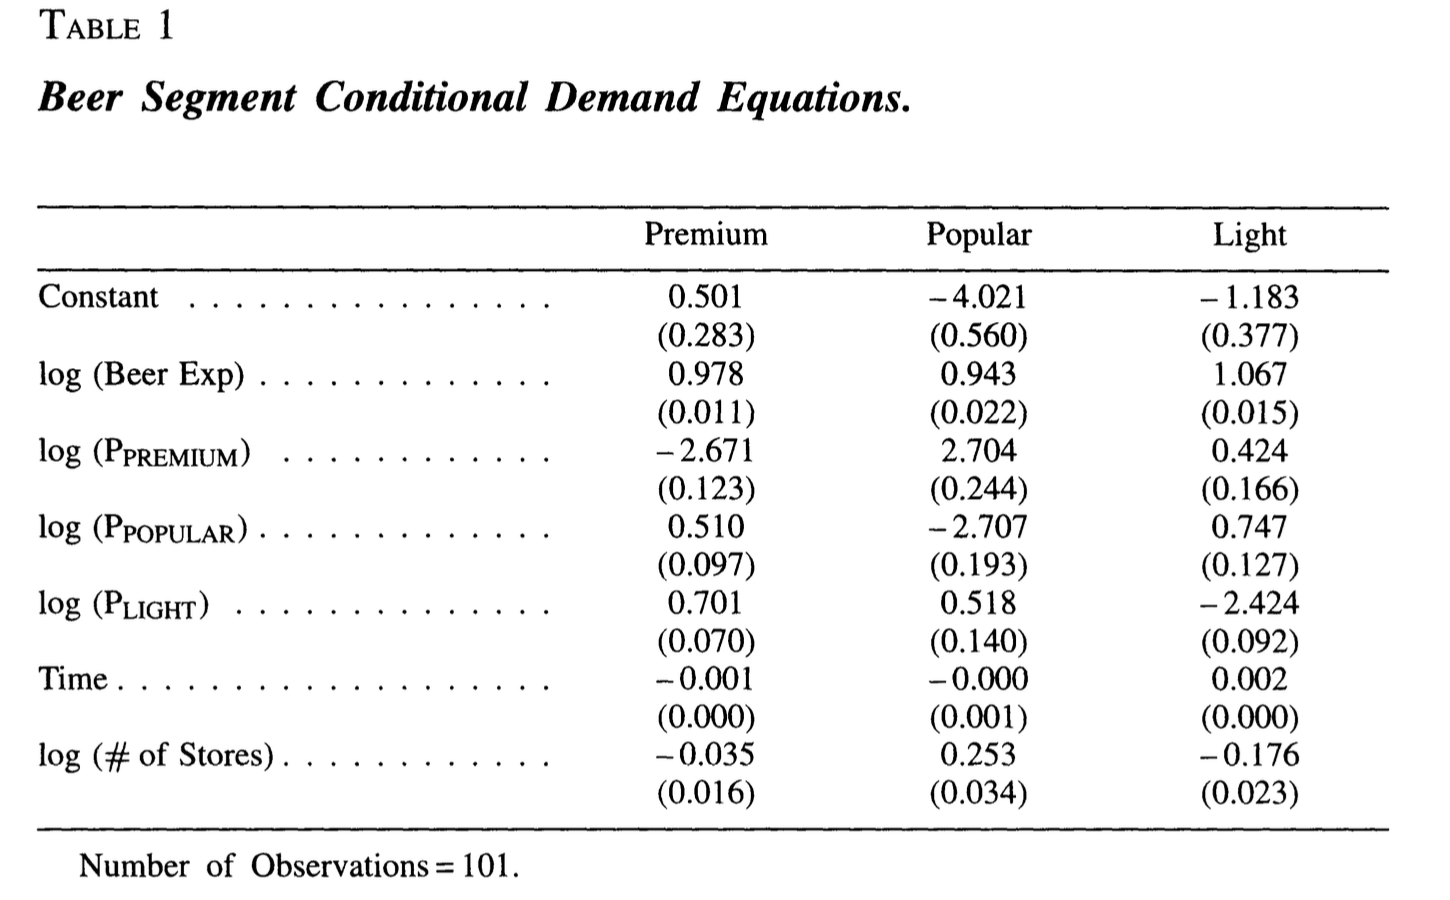
\includegraphics[width=3in]{resources/beer1.png}
\end{center}
\end{frame}

\begin{frame}
\frametitle{Hausman, et.al (1994)}
\begin{center}
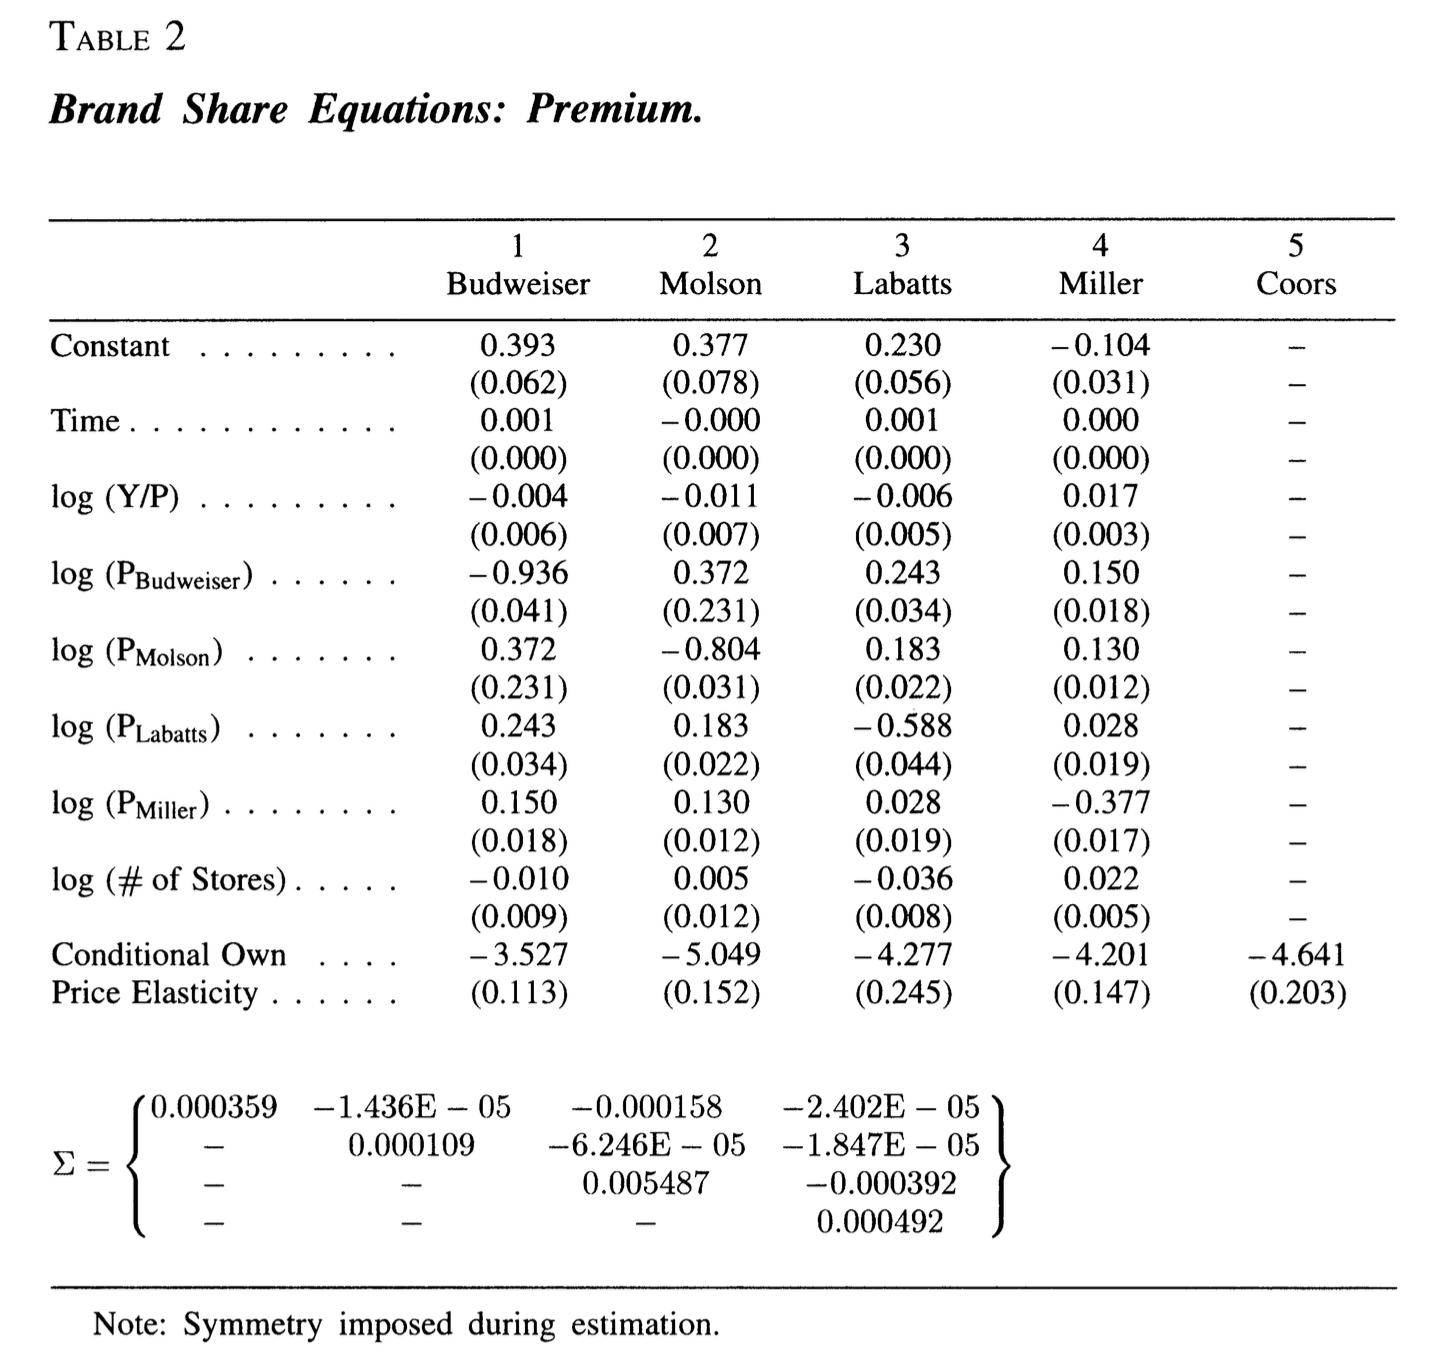
\includegraphics[width=3in]{resources/beer2.png}
\end{center}
\end{frame}

\begin{frame}
\frametitle{Hausman, et.al (1994)}
\begin{center}
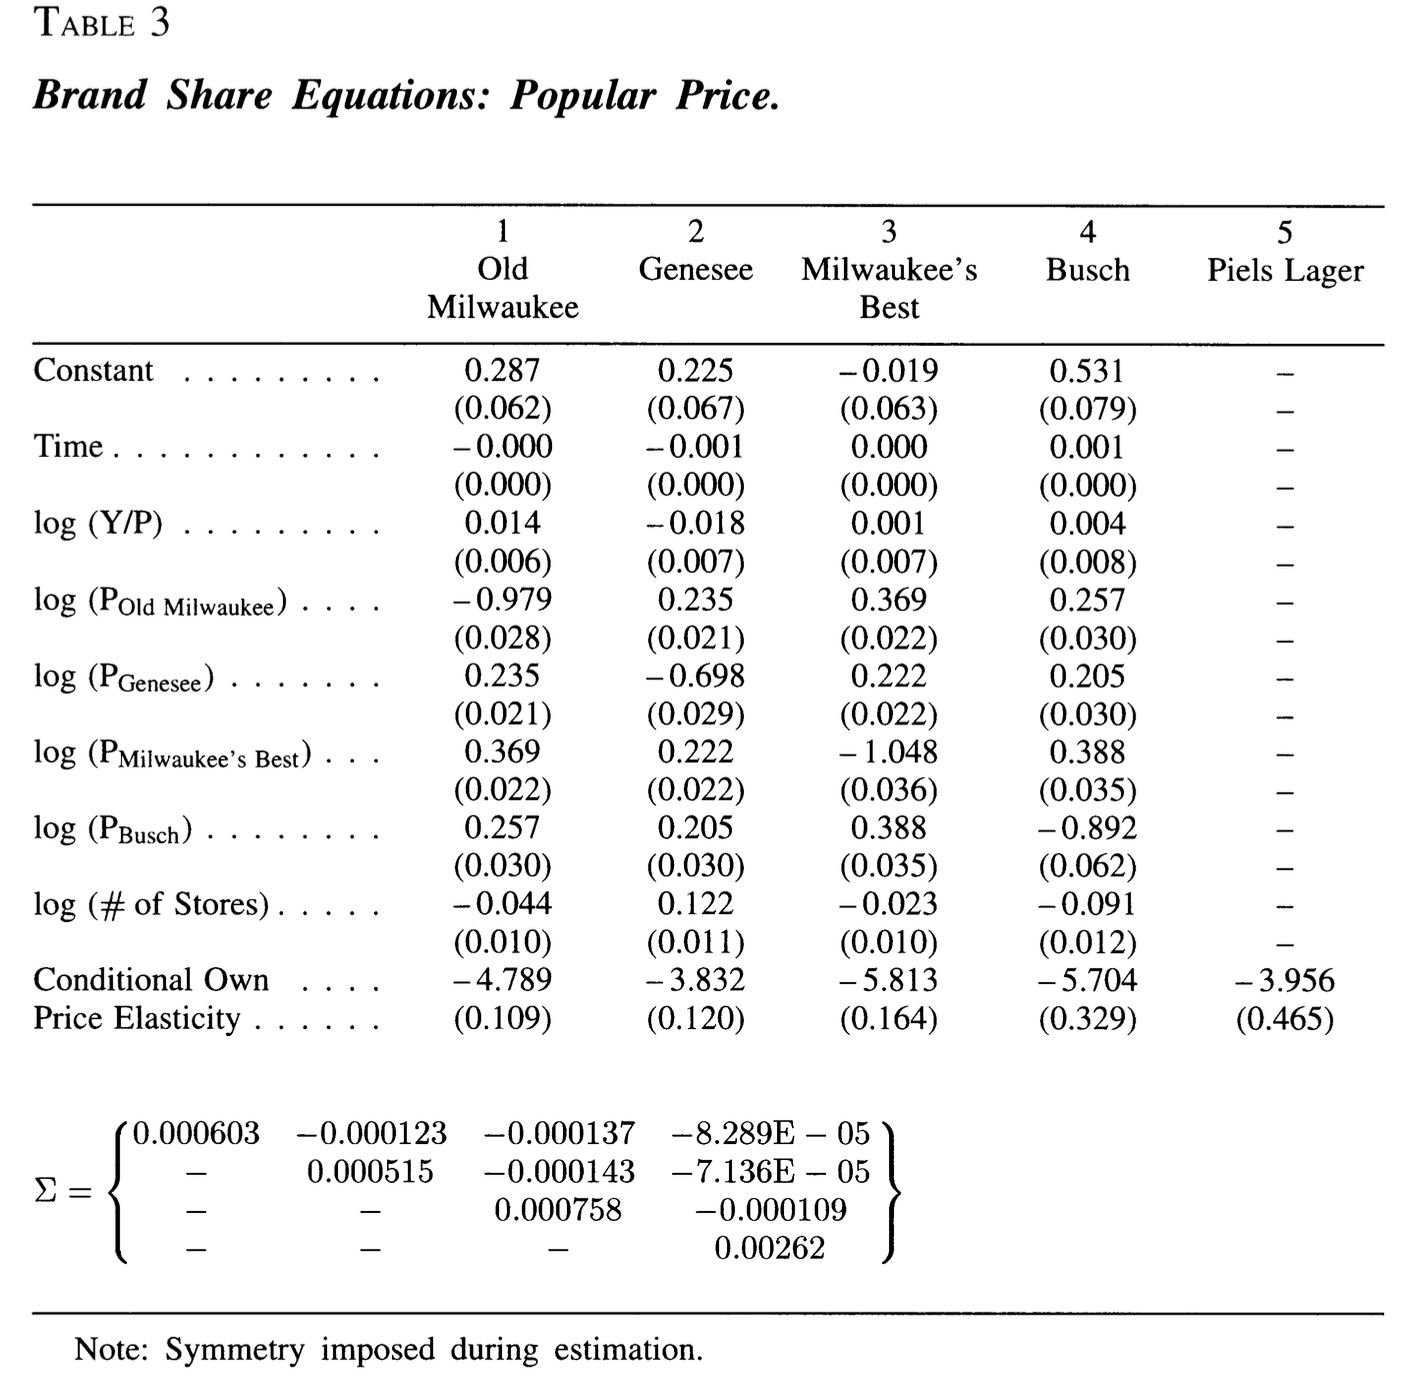
\includegraphics[width=3in]{resources/beer3.png}
\end{center}
\end{frame}

\begin{frame}
\frametitle{Hausman, et.al (1994)}
\begin{center}
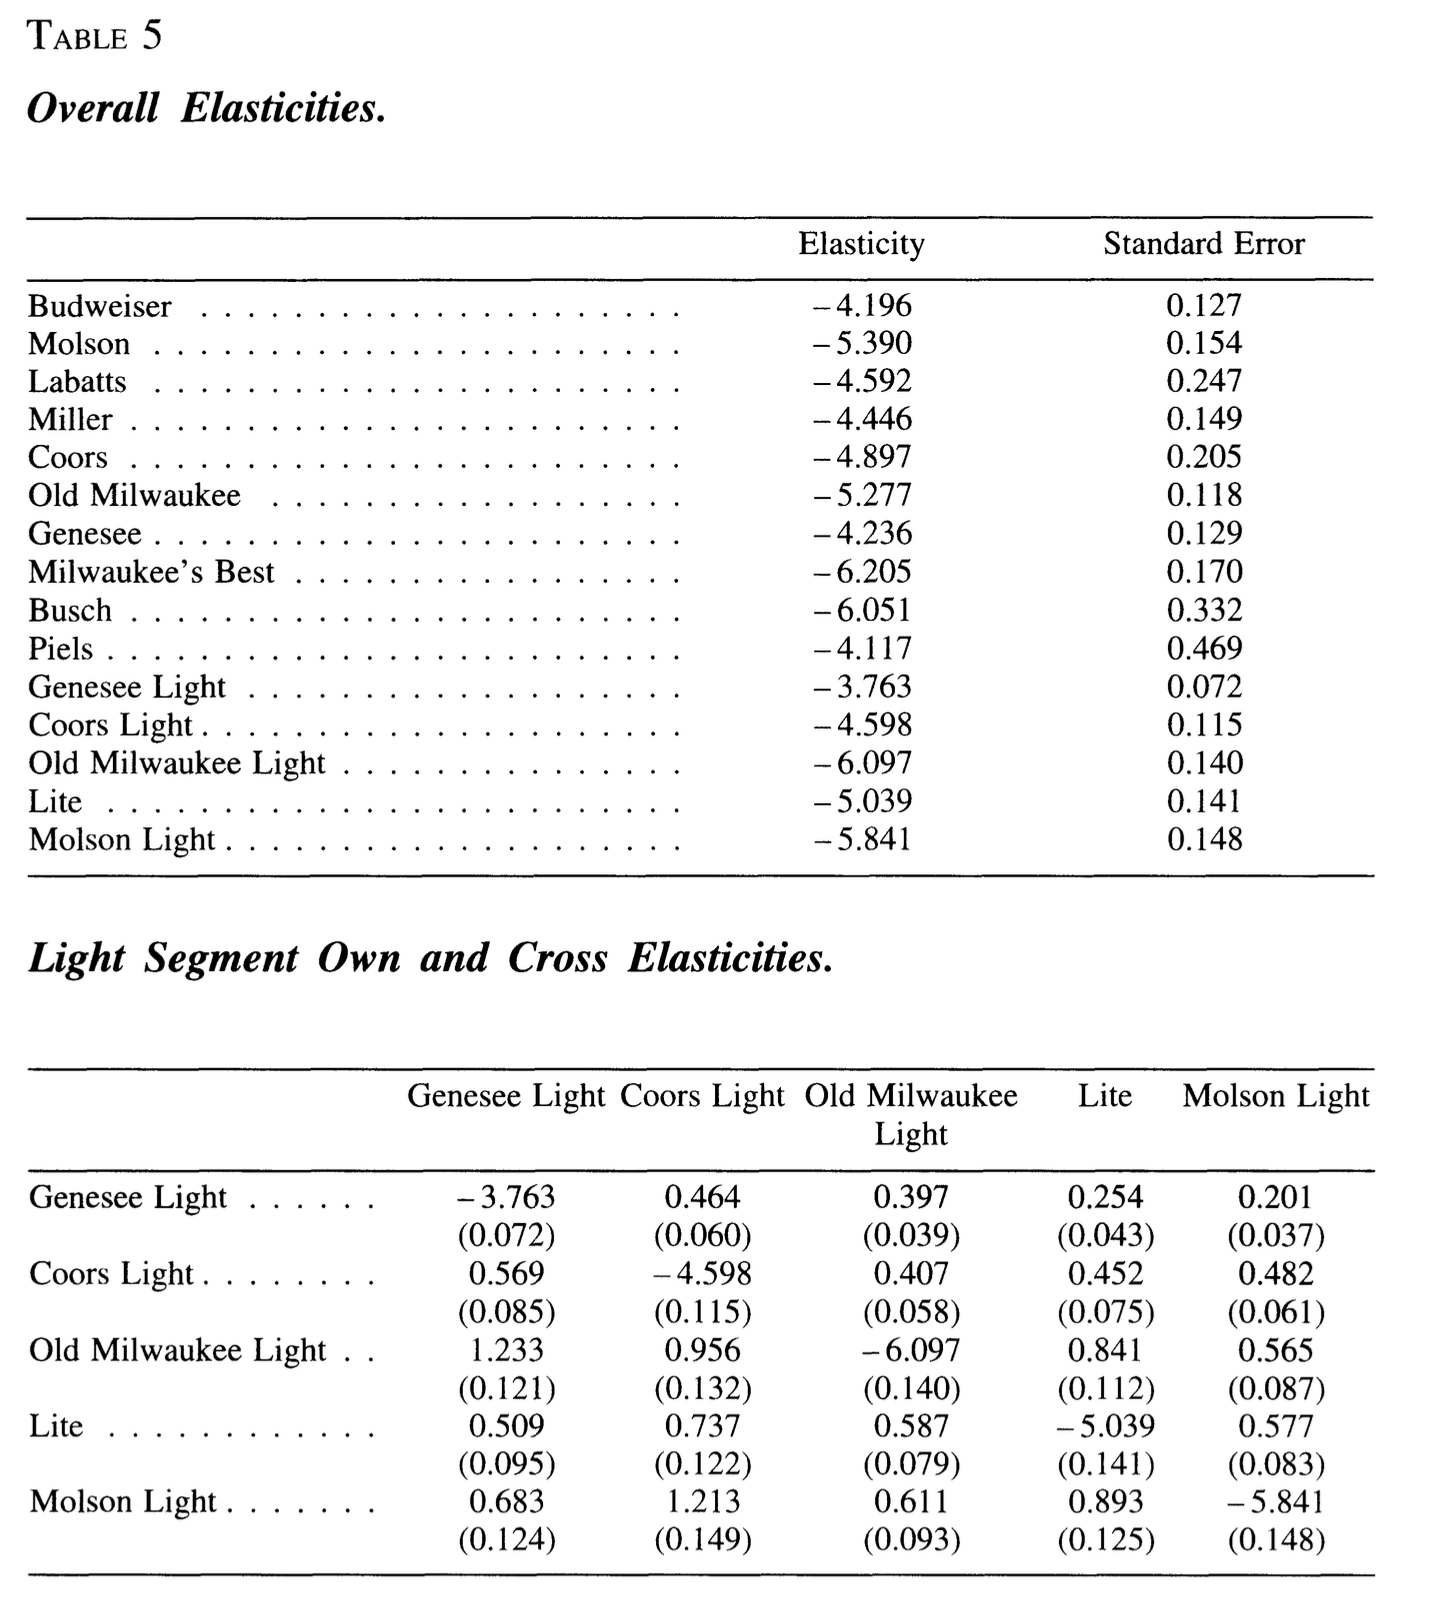
\includegraphics[width=2.5in]{resources/beer5.png}
\end{center}
\end{frame}

\begin{frame}
\frametitle{Hausman, et.al (1994): Results}
\begin{itemize}
\item Relatively large own and cross price elasticities.
\item Authors simulated \alert{partial merger analysis}.
\begin{itemize}
\item Hold prices of all non-merging parties fixed.
\item Solving for best-response of single-product.
\item How would full equilibrium analysis differ?
\end{itemize}
\item  Merger of Coors and Labatt's: Coors Markup 19.9\% $\rightarrow$ 23.2\% (small).
\item Claim is that presence of other competitors constraints potential to raise prices. How? Why?
\end{itemize}
\end{frame}

\begin{frame}
\frametitle{Other AIDS examples}
 Hausman (1997) aka \textit{The Apple Cinnamon Cheerios War}.
\begin{itemize}
\item What is the value of a new good? How should we adjust CPI?
\item Potentially HUGE issue. Why?
\item Weekly cereal data.. 7 cities, 137 weeks. Three segments (adults, kids, family) with max 9 brands.
\item Calculate $e(p_{-n},p_n^*,u) / e(\mathbf{p},u)$. Find a \alert{virtual price} $p^{*}$ (or choke price) that leaves consumers as well off as a world without Apple-Cinnamon Cheerios.
\item Virtual price is about $2 \times$ actual price. CPI may be overstated by as much as 25\% for all cereal brands (tons of new products).
\end{itemize}
\end{frame}

\begin{frame}
\frametitle{Other AIDS examples}
 Chaudhuri, Goldberg, Jia (AER 2006)
\begin{itemize}
\item Indian market for antibiotics: (foreign vs. domestic) (licensed vs. unlicensed producers).
\item Different brands, packages, etc. also different active ingredients ($J=300$ they aggregate to four active ingredients $\times$ country of origin).
\item Monthly sales data (SKU level) for 4 regions in India (Market Research firm).
\item What would prices and quantities look like if intellectual property rights were enforced and unlicensed producers were shut down?
\end{itemize}
\end{frame}

\begin{frame}
\frametitle{Chaudhuri, Goldberg, Jia (AER 2006)}
Issues
 \begin{itemize}
\item Products enter and exit the market. How do we model this?
\item Dosages differ across products. How do we construct $Q$?
\item Don't treat licensed v. unlicensed as different products. Why?
\end{itemize}
Results
 \begin{itemize}
\item Estimate AIDS demand aggregated across demands
\item Get upper and lower bounds on marginal costs
\begin{itemize}
\item Assume that $p=mc$
\item Assume monopoly pricing.
\end{itemize}
\item Calculate the \alert{virtual price} or ``choke price'' that makes expenditures zero on unlicensed products.
\item Get changes in consumer surplus (integrated demand curve) and producer profits without unlicensed firms.
\end{itemize}
\end{frame}


\end{document}
